\documentclass[12pt]{article}
\usepackage[final]{graphicx}
\usepackage{times}
\usepackage{relsize}
\usepackage{microtype}

\usepackage{alltt}
\usepackage{url}
\usepackage{comment}
\usepackage{relsize}
\usepackage{floatflt}

\usepackage{geometry}

\geometry{verbose,papersize={8.5in,11in},
  left={1in},width={6.5in},top={1in},bottom={1in}}

\begin{document}
\title{
       Department of Information and Computer Sciences\\
       {\bf Review of Provisional Ph.D. Program} \\
       University of Hawaii at Manoa}

\maketitle

\tableofcontents

\newpage

In this document we provide the information requested in {\em Appendix D:
Guidelines for Assessment of Provisional and Established Programs} for the
Information and Computer Sciences Ph.D. program.

\section{Assessment of need factors}

Because it provides a useful introduction to the value and importance of the ICS
Ph.D. program, we begin this report by responding to the final requested
item of information in Appendix D.

{\em
\medskip \noindent In the case of graduate programs, attention should also be given to the
following need factors:
\begin{itemize}
\item The direct relevance of the contribution of the field of study to the
  professional, economic, social, occupational and general educational
  needs of Hawaii; 
\item A ``national needs factor'' that emphasizes the direct relevance of
  the contributions of the field of study to national needs and where
  Hawaii and the University have unique or outstanding resources to
  respond with quality;
\item An ``international needs factor'' the emphasizes the direct relevance of
  the contributions of the field of study to international needs and where
  Hawaii and the University have unique or outstanding resources to
  respond with quality;
\item An educational needs factor the indicates the direct relevance of the
  field of study to basic education needs for which there is a demand by
  Hawaii's population;
\item The relevance of a field of study as a necessary supporting
  discipline for quality programs identified by the above criteria;
\end{itemize}
}

\subsection{International need factors}

Computer science is a fundamental discipline whose advances in research and
development impact the lives of millions of people every day across the globe. In 2009, a
panel of 8 experts from the Wharton School of Business (University of
Pennsylvania) was asked to name the 20 biggest innovations of the last 30
years, with the results published in the New York Times in March of that
year. Out of the 20 innovations, 9 are directly from the field of computer
science (the Internet, person computers, email, the microprocessor, office
software, open source software, e-commerce, media file compression, and
social networking) and 5 of the remaining 11 are directly enabled by it.

Given this impressive coverage, it is not surprising that computer science
Ph.D. programs are mainstays of virtually all first tier research
universities worldwide.  What makes computer science unique is its
cross-cutting impact and relevance for other disciplines. Indeed, computers
are used today not only in virtually all disciplines of science and
engineering (where computer modeling and simulation are pervasive), but
also in all the humanities (e.g., due to the use of large-scale and
distributed digital databases), with direct involvement in fields as
diverse as education (e.g., for internet collaboration technologies for
learning) and even music (e.g., for computer-aided composition).  Far from
being straightforward applications of computers, many important
developments in those fields require that computer science challenges be
addressed through innovative research and development activities, such as
those pursued by ICS Ph.D. students.  Consequently, advances in computer
science research are fundamental for furthering human knowledge and
progress in general.

\subsection{University need factors}

Since computer science's relevance is pervasive across so many disciplines,
our Ph.D. program is an invaluable resource for the university:

\begin{itemize}

\item ICS Ph.D. students are often engaged in collaborative projects
  between professors in ICS and in other departments.  They are thus key
  contributors to the fostering of interdisciplinary research at UHM, which
  is highly strategic given the amount of federal funding available for
  such research.

\item A significant fraction of our Ph.D. students are currently or
  were previously supported by Research Assistantships hosted in other
  departments. This is because many research projects require the type of
  expertise that only our students have through the training
  provided in our Ph.D. program. We regularly receive 
  requests from Principal Investigators on campus asking us to advertise
  Research Assistantship opportunities to our graduate students. Thus, our
  Ph.D. students provide a unique and important research workforce for the
  university.

\item Our graduate program offers courses that provide advanced training
  for graduate students outside of our programs. Every semester, such
  students take our graduate-level courses. For instance, Oceanography and
  Astronomy students have take our high-performance computing course,
  Biology students have taken our bioinformatics course, Educational
  Technology students have taken our Human-Computer Interaction courses.

\item Almost 30\% of our Ph.D. graduates to date have chosen to stay in the
  University of Hawaii system and contribute either to research and
  development activities or to information technology management.
\end{itemize}

\subsection{Hawaii need factors}

Innovations in computing through Ph.D. research drive economic growth for
the state of Hawaii. This growth occurs not just in the IT industry, but
across the entire economy.  A strong computer science Ph.D. program
provides a nexus for this growth and the means to both build Hawaii's
capacity for technical innovation and to staff Hawaii’s research and
development community.  In the specific case of Hawaii, the benefit goes
beyond economic growth to (much needed) economic
diversification. Consequently, a strong ICS Ph.D. program can be a major
contributor to growing a diversified economy in Hawaii.

The career paths of our Ph.D. graduates is a clear testimony of the
dramatic impact that our students have on the state's
economy. Approximately 35\% of our Ph.D. graduates so far have chosen to
stay in Hawai`i and work in local research and development organizations.
The impact of these graduates is also felt at the level of the community.
As just one example, many of our Ph.D. students are active contributors to
TechHui, Hawaii's premier social network for science, technology and new
media.

Our Ph.D. program fulfills a clear local educational need. For instance,
for Fall 2009 admissions, out of the 17 applicants to our Ph.D. program, 4
were local to Hawaii.  Out of these 4 applicants, 3 were admitted to our
program. These are outstanding local students who were exposed to research
during their undergraduate experience at the University of Hawaii, and
although many alternatives were available to them, they chose our
Ph.D. program based on their interactions with our faculty and the
opportunities this degree would make available to them.

In summary, the national and international need for computer science
Ph.D. graduates is currently strong and will only grow stronger in future.
Regionally, the diversification of the Hawaii economy requires skilled,
innovative thinking in high technology areas which computer science
Ph.D. graduates are ideally suited to provide.  Finally, the ICS
Ph.D. program provides students who are in high demand and a valued
resource to other departments.   

We believe strongly that the ICS Ph.D. program satisfies university, state,
national, and international need factors. 

\section{Assessment of program organization and objectives}

{\em Following the guidelines in Appendix D, this section discusses the ICS
  Ph.D. program curriculum, requirements, advising, and counseling, with
  the goal of establishing that the ICS Ph.D. program is organized in such
  a way as to meet its objectives. }

\subsection{Objectives}

The Ph.D. is the highest degree awarded by universities in the United
States and thus represents the pinnacle of academic achievement.  The Ph.D.
Program in Information and Computer Sciences is designed for students who
want to contribute to the study of the description and representation of
information and the theory, design, analysis, implementation, and
application of algorithmic processes that transform information.

ICS Ph.D. students receive advanced training in the scientific principles and
technology required to develop and evaluate new computer systems and
applications. We equip our students with the expertise necessary to
independently perform state-of-the-art research, to formulate and develop
creative solutions to novel and existing problems, and to intelligently
manage the research of others. Our curriculum covers all major areas of
computer science, with active research in areas including artificial
intelligence, bioinformatics, human-computer interaction, software
engineering, machine learning, high performance computing, digital
democracy, computer vision, and computer systems.

An applicant may be admitted with a Bachelor's degree or with an
M.S. degree in computer science or a related field. If the applicant enters
without the M.S., the applicant will earn the M.S. before proceeding to the
"Ph.D. portion" of the program.

The ICS Ph.D. curriculum is designed to: (1) Certify the student's core
competency in computer science and address any deficiencies in this
competency as efficently as possible, so that the bulk of the student's
Ph.D. program is focused on research. (2) Prepare the student to do
research through an apprenticeship with a faculty member, assessing
readiness to do research with a research portfolio that is analogous to a
professional tenure and promotion portfolio.  We achieve these goals by
guiding the students through a curriculum with the following components:
(1) Demonstration of core competancy; (2) Participation in ICS 690; (3)
Preparation of a research portfolio; (4) Proposal defense; and (5) Final
defense.

\subsection{Demonstration of core competency}

The ICS Ph.D. student will demonstrate core competency in computer science
by meeting the following two requirements:

\begin{enumerate}
\item Completion of a Master's degree in Computer Science or a related
  field, where what counts as ``related'' is at the discretion of the
  graduate program chair, assisted by the admissions committee;
\item Successful completion of the comprehensive exam.  The comprehensive exam
  covers core knowledge of computer science at a level that might be
  reasonably expected of a job interviewee with a Master's degree.
  Students shall take the comprehensive exam at the end of the first semester
  of the the Ph.D. portion of their students.  Students may attempt the
  comprehensive exam only twice, and must pass this exam no later than the end
  of the first year of their Ph.D. studies.  
\end{enumerate}

\subsection{Coursework}

According to Graduate Division guidelines, coursework is optional for
University of Hawaii Ph.D. programs.  However, the ICS Ph.D. program
requires all ICS Ph.D. students to attend and pass the seminar course ICS
690 each semester they are in the program.  ICS 690 is a one credit seminar
course that meets once a week and is directed by the Graduate Chair. It
provides an opportunity for all ICS graduate students (both M.S. and Ph.D)
to regularly discuss their research issues and problems and gain insight
from presentations by other faculty members, other graduate students, and
guest lectures by visiting academic and industry professionals.  

\subsection{The research portfolio}

By the end of the year following the passing of the comprehensive exam, the student
must prepare and submit a research portfolio that includes the following:

\begin{enumerate}
\item A statement of purpose, which is a one to two page description of the
  student's professional interests in research, teaching, service, and/or
  product development;
\item Evidence of core competancy, as described above;
\item Evidence of scholarly ability, i.e. the ability to identify,
  critically analyze, and research a problem, and of written communication
  skills, in the form of two items authored by the student and reviewed by
  doctoral level scholars. The first item is a written literature review in
  the proposed area of study of 20-30 pages, following the graduate
  division dissertation format and reviewing at least 20 published
  works. The second item must be one of the following:  a masters thesis by
  the student; a publication by the student in a reviewed conference or
  journal; or a technical report approved by at least two other faculty
  members. 
\item (Optional) Other evidence of professional capacity, which might
  include a professional vita of employment, professional presentations, reviewing of papers for conferences and journals, competitive fellowships, patents, teaching, and service on committees or as graduate student representatives contribute to the candidacy decision. Letters of reference may also be included. Students should report all forms of research, teaching, and service to the community and to the discipline when preparing their portfolios.
\end{enumerate}

The portfolio is approved by a two-thirds majority vote of a quorum of the ICS faculty (typically at a faculty meeting). The portfolio shall be distributed to the faculty in advance of the meeting at which it will be voted upon.

The graduate program chair shall designate one faculty to argue for the student's case and one to argue against the student, who may both vote as they see fit. Faculty that have a conflict of interest with the student (e.g., advisor or co-advisor, co-author on research articles, direct supervisor) cannot serve in these capacities.

The portfolio must be approved before undertaking the Proposal Defense.

\subsection{Proposal defense}

Before commencing the final dissertation research, the student shall give a
public defense of his or her Ph.D. proposal. Students prepare a research
proposal that includes a literature review in the chosen topic area (this
usually is but is not required to be derived from the literature review
from the portfolio) and a description of research topics to be
investigated. This work should be done under the direction of an
appropriate faculty adviser.  Students must also form their dissertation
committee prior to the proposal defense.

The defense includes both a presentation of the student's research
proposal and an oral examination covering their general preparation for the
research involved, as specified in the General and Graduate Information
Catalog.

It is generally advised that the proposal defense be scheduled for a time period of 3 hours. 

Once the student passes the proposal defense, they then conduct their
research and write a dissertation under the direction of their advisor and
their dissertation committee.

\subsection{Final defense}

The final defense is a public presentation of the student's completed
research and dissertation.  The dissertation must be presented to and
approved by a doctoral committee, as specified in the General and Graduate
Information Catalog.

We believe that our five step process of demonstrating core competancy,
participation in ICS 690, preparation of a research portfolio, proposal
defense, and final defense, when combined with our graduate curriculum and
research areas, creates an effective and efficient program for students who
wish to contribute to the study of the description and representation of
information and the theory, design, analysis, implementation, and
application of algorithmic processes that transform information. Our
program is thus organized in such a way as to meet its objectives.


\section{Assessment of student learning objectives}

{\em Following the guidelines in Appendix D, this section assesses the
  whether or not the program is meeting its learning objectives for
  students. }

\subsection{Learning objectives}

We have defined nine student learning objectives for the ICS Ph.D. program,
six of which are shared with our M.S. program plus an additional three
learning objectives specific to the Ph.D. program.

The ICS M.S. graduate program provides courses for advanced education in
Computer Science and affords opportunities to conduct research. Our
objective is to help students achieve a high level of professional
competence and lifelong learning, with the following Student Learning
Objectives:

\newcounter{listcounter}
\begin{list}{\arabic{listcounter}.}{\usecounter{listcounter}}
\item Master core computer science theoretical concepts, practices and technologies;
\item Identify, formulate and solve problems employing knowledge within the discipline;
\item Contribute effectively to collaborative team oriented activities;
\item Communicate effectively about computer science topics using appropriate media;
\item Demonstrate advanced knowledge in an area of specialization within the discipline;
\item Engage in significant research in their area of specialization within the discipline and/
or in projects that respond to community and industry needs.
\end{list}

The ICS Ph.D. graduate program provides advanced, individualized training in research 
in Computer Science, preparing students for research careers in academia and industry.  
Beyond  those for the M.S. program, the Ph.D. program involves the three following 
Student Learning Objectives:

\begin{list}{\arabic{listcounter}.}{\usecounter{listcounter} \setcounter{listcounter}{6}}
\item Develop a research portfolio that demonstrates the capacity to carry out original 
research in the field;
\item Become an expert in the area of specialization including mastery of the relevant 
research skills and methods, develop a research vision, and formulate a research plan 
that will lead to novel scientific contributions;
\item Execute a research plan and demonstrate original contributions to the field, as 
shown through findings and/or publications, culminating in a Ph.D. dissertation and oral 
defense.
\end{list}

\subsection{Assessment}

Our development of empirically based assessment procedures for these student learning
objectives is ongoing.  For example, we have planned, but not yet
implemented, an ``exit interview'' procedure in which we can gather data
directly from each graduating student regarding their subjective view as to
whether each of these student learning objectives were achieved. We also
plan to classify each course in the curriculum according to the program
SLOs that it covers, which would provide an additional level of evidence
regarding assessment and coverage by noting which courses the student took
during their program. 

Although development of assessment procedures is ongoing, we believe
strongly that the basic structure of our program as described above ensures
that successful graduates have satisfactorily achieved all of these
learning objectives, as illustrated in Table \ref{phd.slos}.

\begin{table}[htbp]
\begin{center}
\caption{Ph.D. program components and satisfaction of student learning
  objectives}
\label{phd.slos}
\begin{tabular}{|l|l|} \hline
{\bf Ph.D. program component} & {\bf Student Learning Objective(s) Addressed}  \\ \hline
Demonstration of core competancy & 1 \\
Participation in ICS 690 & 3, 4,  \\
Preparation of a research portfolio & 2, 4, 5, 7, 8 \\
Proposal Defense & 1, 2, 4, 5, 6, 8 \\
Final Defense & 1, 2, 4, 5, 6, 8, 9 \\ \hline
\end{tabular}
\end{center}
\end{table}

\section{Assessment of program resources}

{\em Following Appendix D, this section addresses whether or not program
  resources are adequate through an analysis of the number and distribution
  of faculty, faculty areas of expertise, budget and sources of funds, and
  facilities and equipment.}

\subsection{Faculty resources}

In addition to the Ph.D. degree, the ICS department offers the following
degrees: B.A. in ICS, B.S. in Computer Science, M.S. in
ICS, and a MLISc. In addition, we contribute to 2 of the 4 programs
in the interdisciplinary Ph.D. program in CIS, and we offer the BSCE with the
Department of Electrical Engineering.

Table \ref{fig:faculty} shows an overview of the faculty in the unit and
the recent faculty turnover due to attrition. Except for the two ICS/LIS
faculty members (listed as half time) LIS faculty do not participate in the
Ph.D. degree so they are not included in the total numbers for this
report. 

\begin{table}[htbp]
\begin{center}
\caption{ICS faculty resources and attrition}
\label{fig:faculty}
\begin{tabular}{|l|l|l|} \hline
{\bf Faculty} & {\bf Rank/Position} & {\bf Date of Initial Hire} \\ \hline
Martha Crosby & Professor and Chair & 4-1-79 \\ \hline
Philip Johnson & Professor and Associate Chair & 8-1-90 \\ \hline
David Chin & Professor & 1-1-88 \\
Daniel Suthers &  & 8-1-98  \\ \hline
Kazuo Sugihara & Associate Professor & 8-1-85   \\
Jan Stelovsky &                      & 1-29-87    \\
Edoardo Biagioni &                   & 8-1-97   \\
Luz Quiroga (0.5) &                  & 8-1-00   \\
Kimberly Binsted &                   & 1-1-02   \\
Nancy Reed	 &                   & 1-1-02   \\
Susanna Still &                      & 1-1-05   \\
Guylaine Poisson &                   & 1-1-05   \\
Henri Casanova &                     & 8-1-05   \\
Scott Robertson &                    & 8-1-07   \\ \hline
Kyungim Baek &   Assistant Professor & 8-1-05   \\
Richard Gazan (0.5) &                & 8-1-07   \\
Curtis Ikehara	&                    & 8-1-07   \\
Julia Patriarche &                   & 8-1-08   \\
Lipyeow Lim	&                    & 8-1-09   \\ \hline
Gerald Lau &  Assistant Specialist    & 6-15-92   \\ \hline 
\multicolumn{3}{|c|}{ {\bf LIS faculty} } \\ \hline
Diane Nahl & Professor & 8-1-90 \\
Violet Harada & & 8-1-93 \\
Peter Jacso & & 8-1-94 \\
Rebecca Knuth & &  8-1-95 \\ \hline
Andrew Wertheimer & Associate Professor & 8-1-03 \\ \hline
Noriko Asato & Assistant Professor & 8-1-07 \\ \hline \hline
\multicolumn{3}{|c|}{ {\bf Faculty who have left the department} } \\ \hline
\multicolumn{3}{|p{5in}|}{ James Corbett, William Howden, Jintae Lee, Torbin Nielson, Daniel Watanabe,
Hong Hua, Christopher Hundhausen, Isao Miyamoto, Wilbert Gersch, Art Lew,
W. Wesley Peterson, David Pager, Stephen Itoga} \\ \hline \hline
\multicolumn{3}{|c|}{ {\bf Positions lost} } \\ \hline
\multicolumn{3}{|p{5in}|}{ Clerk Typist III} \\ \hline
\end{tabular}
\end{center}
\end{table}

Currently the ICS Ph.D. program is supported by 4 full professors, 9.5
associate professors, 4.5 assistant professors, and 1 educational
specialist in the tenure or tenure track category. The educational
specialist provides academic support by coordinating and assisting the
Department Chair and Graduate Program Chairs in major aspects of student
services, including recruitment, financial assistance, and placement
services. The position also coordinates outreach programs and acts as
liaison with other campus-wide committees, alumni groups and the general
community. We have employed non-tenure track faculty but have lost them due
to budget cuts. The department has also lost 5 senior ICS faculty members since
2007 through death or retirement. We hope to hire faculty that can both
contribute to the Ph.D. program and replace the missing areas of expertise.

The average instructional workload for each faculty member is two courses
per semester. Using the Teaching Equivalent Workload Spreadsheet adopted by
the College of Natural Sciences, we estimate that the faculty averages 8.82
semester credit hours for coursework (including directed reading courses,
thesis advising and guest lecturing) and another 2.10 for additional
teaching, for a total of 10.92 semester credit hours. On February 18, 2011
a comprehensive ICS Department Workload Documentation Procedure was
approved by faculty. It is available for viewing at: http://goo.gl/IGRrr

Our program currently counts 42 graduate students (23 M.S. students and 19
Ph.D. students).  One constraining factor for Ph.D. program size is the
limited (and in some cases dwindling) numbers of Teaching and Research
Assistantships. Such support is essential for attracting and retaining
students.

Currently, all our Ph.D. students are supported.  Growth of the program
would be facilitated by increased availability of support.  Another
constraining factor is the student-to-faculty ratio. Currently this ratio
is about to 2 (i.e., on average a graduate faculty member advises 1
Ph.D. student and 1 M.S.  student), but it was equal to 3 only a couple of
years ago. Such fluctuation is typical and follows fluctuations in
applications and graduations. For instance, many students graduated in
2009, leading to a somewhat lower ratio in 2010.  At any rate, due to our
relatively low student-to-faculty ratio, our students benefit from
intensive advising, which is instrumental to their successful graduations.
To ensure that the quality of the advising remains high, a significant
increase in the student population would require an increase of our faculty
as well.

\subsection{Administrative resources}

In addition to the instructional staff, the department has two information
technology (IT) specialists. They are responsible for system
administration, networking, installation, and maintenance of the
department’s computer hardware and software infrastructure. The IT
specialist also researches software and other products in response to
instructional and research needs and manages the purchasing and budget
maintenance for the department. In 1998 we hired Nolan Oshiro as a Computer
Specialist 111 to manage our Computer Labs and to manage our networking
environment. Andreas Koga was hired to assist Nolan and replace previous
staff that left the department. Nolan and Andreas efficiently manage the
department facilities with the help of student assistants. The department
also hired Michael-Brian Ogawa, a specialist who manages the several
sections of ICS 101 with the help of several student assistants. The
department employs 12 teaching assistants. Departmental research efforts
have produced several grants which employ student research assistants.

Wesley Sugimoto provides administrative and fiscal support to the
Department of Information and Computer Sciences. He works with the
Department chair to develop and track an annual department budget with
corresponding projections for all sources of revenues including general and
all extramural funds. He assists faculty with budgetary matters related to
grant and contract proposals. He works with faculty and funding agencies
(NSF, DARPA, etc.) to obtain the necessary application and reporting
forms. He generates timely fiscal status reports to meet the needs of the
college, department, accreditation bodies, and researchers. He works with
clerical staff to insure prompt and accurate payment of obligations to
vendors upon delivery of goods and services.

Janice Oda-Ng, a Secretary II, performs secretarial and administrative
duties for the Department, including work relating to curriculum and
instruction and personnel as well as services relating to the clerical and
administrative needs of the faculty members of the Department.

\subsection{Program resources}

The computer science department receives an annual budget assigned by the
College of Natural Sciences. This budget supports operational costs such
as:
\begin{itemize}
\item Office Supplies
\item Software Subscriptions
\item Course Note Duplication
\item Spare Parts
\item Software Licenses
\item Hardware and Hardware Repair Costs
\item Minor Facility Renovations
\end{itemize}

In addition, in Fall 2001, the ICS Department was given a legislative
appropriation of \$1 million to supplement our instructional budget for AY
2002. However, this appropriation was intended to support development of
undergraduate courses and thus does not impact directly on the resources
available for the ICS Ph.D. program. 

\subsection{Staff support and facilities}

Faculty draft most of their own clerical paperwork and send it to support
staff for formalization. Departmental support is primarily in the form of
processing personnel paperwork, formalizing schedules, and ordering
textbooks. The College of Natural Sciences Division provides a review of
grants and fiscal matters. 

\subsection{Research areas and groups}

Table \ref{fig:research-areas} presents areas of research actively pursued
by ICS Faculty members. 

\begin{table}[htbp]
\begin{center}
\caption{ICS faculty research areas}
\label{fig:research-areas}
\begin{tabular}{|lll|} \hline
 Algorithms & Artificial Intelligence & Robotics \\
 Biomedical Informatics & Bioinformatics & Collaborative Systems \\
 Compilers & Computational Neuroscience & Computer Vision \\
 Databases & Human Computer Interaction & Library and Information Science \\
 Machine Learning & Mathematical Finance & Mobile Computing \\
 Ubiquitous Computing & Renewable Energy & Security \\
 Information Assurance & Software Engineering & Systems \\
 Networking & High-Performance Computing & Computer Learning \\ \hline
\end{tabular}
\end{center}
\end{table}

In addition, faculty have organized a variety of research laboratories to
support larger, collaborative, and potentially interdisciplinary research
projects.

\medskip\noindent The {\bf Adaptive Multimodal Interaction (AMI) Laboratory} supports
research involving various metrics and methodologies to study user
data. Typical experiments collect eye movements, pressure grasping, and
other physiological input to develop novel and effective interactive
systems.  Research in this area has fostered new design principles, user
interfaces, multimedia interaction systems, and visualizations of complex
information

\medskip\noindent The {\bf Bioinformatics Laboratory (BIL)} supports Bioinformatics and
Metagenomics projects.

\medskip\noindent The {\bf Collaborative Software Development Lab (CSDL)} has pursued
well-funded research leading to innovative software technologies in use by
many academic and industrial sites worldwide.  Currently they are involved
in renewable energy research. 

\medskip\noindent The {\bf Concurrency Research Group (CORG)} pursues research in  parallel
and distributed computing, computer system simulation, and high-performance
computing.

\medskip\noindent The {\bf Hawai'i Computer-Human Interaction (HI'CHI) Laboratory} focuses on
understanding how people use information systems and is dedicated to
informing design based on human performance data. Current research on
digital government applications and how people use the Internet to make
political decisions.

\medskip\noindent The {\bf Laboratory for Interactive Learning Technologies (LILT)} is
forging partnerships with the Department of Education and other local
educational agencies to support innovative uses of high technology in
education.

\medskip\noindent The {\bf Machine Learning (ML) Laboratory} supports machine learning,
robotics and computational neuroscience projects.

\medskip\noindent The {\bf Research Center for Information Assurance (RCIA)} provides a
learning laboratory and test bed for investigations and applications
related to the generation, organization, access, preservation, and secure
use of digital information.


In conclusion, we believe that current resources are sufficient for the
current size of the Ph.D. program, but that growth of the program will be
challenging without recovery of lost resources.




\section{Assessment of program efficiency}

{\em Following Appendix D, this section assesses productivity and
  cost/benefit considerations within the overall context of campus and
  University ``mission'' and planning priorities.  It can include
  quantitative measures comparing SSH/faculty, average class size,
  etc. with other programs in the college, campus, or as appropriate other
  universities.}

We will assess these issues in two ways, through the use of the Academic
Program Cost and Revenues template and through a time-to-degree analysis.

\subsection{Academic program cost and revenues}
\label{sec:costs}

\begin{figure}[ht]
  \center
  \includegraphics{costs.eps}
  \caption{\em \small Academic Program Cost and Revenue Template}
  \label{fig:costs}
\end{figure} 

Figure \ref{fig:costs} presents an illustration of the Academic Program
Cost and Revenues Template spreadsheet, filled out according to the
supplied instructions.  This spreadsheet provides a partial, imperfect
perspective on the costs and revenues associated with our Ph.D. program by
showing the overall costs and benefits for our graduate degree program as a
whole (where the numbers include both M.S. and Ph.D. students).

The reason why this spreadsheet provides an imperfect perspective is
because although Ph.D. students are technically not required to take any
classes other than ICS 690, many can and do take advantage of our
curriculum during their Ph.D. program.  Unfortunately, we are not able to
provide the precise values for the SSH associated with just those students
in the Ph.D. program at the point at which they have gone beyond their
M.S. program. Instead, this spreadsheet provides a more general perspective on costs and
revenues associated with our graduate program. 

\subsection{The Ph.D. program as virtuous circle}
\label{sec:virtuous-circle}

We can make a more qualitative, yet more useful argument regarding the
Ph.D. program cost and revenues.  This argument is that the incremental
cost of the program to the department is extremely minimal: essentially,
just the cost of faculty advising for the Ph.D. students, and a fraction of
the cost of ICS 690 (since it is also taken by our M.S. students, so the
Ph.D. students constitute less than half the enrollment.)

On the other hand, the revenue associated with the Ph.D. program is
substantial, because the Ph.D. program supplies students who amplify the
ability of our faculty to produce quality scientific findings.  These
findings, in turn, increase the ability of our faculty to obtain external
funding.  In addition, the presence of a Ph.D. program, and the quality of
our students, help us attract higher quality ICS faculty than we would be
able to without the program.  These higher quality faculty produce higher
quality scientific findings, leading to increased ability to obtain
external funding.  To close this ``virtuous circle'', the increased
external funding provides opportunities to fund new Ph.D. students, who
further amplify the ability of our faculty to produce quality scientific
findings.  Section \ref{sec:reputation} provides quantitative data on the
funding and publications enabled by this virtuous circle.


\subsection{Time to degree}

An alternative measure of program ``productivity'' or ``efficiency'' for
our Ph.D. program is time-to-degree (TTD).  While the TTD can be predicted
fairly accurately for students in M.S. or undergraduate programs (depending
on whether they are full-time students or whether they have full-time
jobs), the same cannot be said of the TTD for a Ph.D. program. This is due
to the original research component, whose duration depends both on the
student and on the chosen area of research within Computer
Science. Variations among students in terms of one year or more is thus
common. Furthermore, some Ph.D.  students are admitted in our program right
after obtaining their B.S., while others come into the program with a
M.S. in hand, which shortens their TTD by at least 1 year and typically 1.5
years if that degree is in Computer Science or a related field.

According to data collected by Graduate Division, the mean TTD in our
Ph.D. program is 5.8 years, with a median of 6.0 years. We can attempt
a comparison with national averages. The report \emph{Time
To Degree of U.S. Research Doctorate Recipients} available from the
National Science Foundation (NSF) Web
site~\footnote{http://www.nsf.gov/statistics/infbrief/nsf06312}
presents data specific to Computer Science programs for academic year
2003. It reports mean ttd between 8.3 and 15.1 years depending on
student categories (Research Assistants, Teaching Assistants,
supported by fellowships, unsupported). The registered-to-degree (RTD)
metric is also reported, which accounts for time during which the
student is actually registered in graduate school, and which ranges
between 7.0 and 9.0 depending on the student category. These times are
``since obtaining a Bachelor.'' We can thus see that our program
compares favorably to nationwide averages, even accounting for the
fact that the Graduation Division data does not account for M.S.
degrees obtained in other institutions.  A recent report on nationwide
doctorate recipients is also available from the NSF Web
site~\footnote{http://www.nsf.gov/statistics/nsf10309}. It presents
data for the 2007-2008 academic year, but unfortunately does not
present data specific to Computer Science programs. Instead is shows
aggregate data for ``Physical Sciences.'' A median TTD of 6.7 years is
reported, which seems to confirm the above observations regarding our program.

The conclusion is that our program allows students to graduate at the
same or at a faster pace than the national average.  While this is good
news, we still see some students who graduate in more than 8 years and up
to 9.5 years. To try to reduce the maximum time to graduation, in 2005
we have redesigned our Ph.D. program.  Like many high-profile programs
nationwide (UC Berkeley, Univ.  of Washington, UC San Diego, etc.) we
have done away with the traditional comprehensive exams.  Instead, in
a view to engaging doctoral students in research as soon as possible,
we have put in place qualifying exams early on and a ``research
portfolio'' exam instead of the comprehensive exams. We thus expect to
maintain our relatively low average TTD but also to reduce our maximum
ttd in the future. Our first graduate for the redesigned program, Mark
Stillwell, successfully defended his dissertation in 2010. He
graduated in 4 years (he already held a M.S. degree in
Mathematics prior to applying to our program), has a very strong
publication record, and has already found a post-doctoral position with
a view to starting a promising Computer Science academic career.


\section{Assessment of program quality}

{\em Following Appendix D, this section assesses the program with respect
  to student performance, satisfaction, placement and employer
  satisfaction, awards to faculty and students, etc.}

\subsection{Department reputation}
\label{sec:reputation}

The ICS department has a national and international reputation and our
faculty have achieved many accomplishments over the years, including
grants, fellowships, awards, contracts and commissions. The ICS faculty
have productive research records and are involved in developing information
enterprises, hold technological patents and have engaged with the community
through consulting, public lectures, and presentations. 

Faculty in the ICS Department have been awarded millions of dollars in
external funding from both industry and government sources.  They serve as
editors on prestigious journals in their areas of expertise, have had their
papers selected as the best paper at conferences, and have won prestigious
awards.  For example, W. Wesley Peterson was awarded the Japan Prize for
his invention fo the Cyclic Redundancy Check (CRC), a fundamental advance
in error correcting codes. Kimberly Binsted, David Pager, Curtis Ikehara,
Martha Crosby, Julia Patriarche, and Jan Stelovsky have all been awarded
patents for their innovations.

Figure \ref{fig:pubs-and-grants} provides a perspective on department
quality based upon the aggregate value of external funding that ICS faculty
have been awarded as PIs or co-PIs, along with the number of refereed
publications that ICS faculty have authored or co-authored.  This is a
snapshot of ICS departmental trends for the four year period of 2006 to
2009, and was generated through review of faculty curriculum vitae and
online sources.

\begin{figure}[ht]
  \center
  \includegraphics[width=0.8\textwidth]{pubs-and-grants.eps}
  %\includegraphics{pubs-and-grants.eps}
  \caption{\em \small ICS publications and funding, 2006-2009}
  \label{fig:pubs-and-grants}
\end{figure} 

Figure \ref{fig:pubs-and-grants} shows that overall aggregate external
funding in which ICS faculty were directly involved varied between \$3M per
year and \$4.5M per year during this four year period, and the number of
refereed publications by ICS faculty varies between 35 and 45 per year.
This data shows that ICS faculty are productive, generating scientific
contributions through refereed publications and helping to bring
significant amounts of external funding to the university. In Section
\ref{sec:virtuous-circle}, we explain why we feel the ICS Ph.D. program
creates a ``virtuous circle'' that supports and grows the ability of our
department to generate funding and scientific advances. 


\subsection{Student application trends}

The average GPA of students joining our Ph.D. program over the last 5 years
is a high 3.82. The percentage of applicants that we accept in our program
has ranged between 38\% and 88\%. The last two years have had inordinate
high acceptance rates above 80\%. In fact, our acceptance rates have
increased steadily throughout the years. While this increase could be
attributed to a lowering our our admission standards, this is absolutely
\emph{not} the case. In fact, our faculty have been absolutely amazed at
the rising quality of applicants to our Ph.D. program in the last could of
years, leading to accepting 15 out of 17 applicants in 2009-2010. This
increase in quality might in part be due to the fact that our Ph.D. program
is recent and is just gaining momentum with our graduates beginning to make
an impact.  The percentage of accepted applicants who eventually join our
program has ranged between 12.5\% and 60\% over the years. Remarkably, in
the last two years, which have seen unprecedented top quality applicants,
50\% and 60\% of these applicants have joined our program. As discussed
below, we do not believe this represents a drop in standards, but rather an increase
in the reputation and stature of our program as it matures.

The data collected by Graduate Division regarding the drop rate for
our Ph.D. program is misleading because it
accounts only for students admitted between Fall 1989 and Spring 1999.
This was when our program was in its infancy and the data is 
for 3 students only.  With the help of a Graduate Division IT
Specialist, on 8/30/2010 we obtained a full history of students in our
Ph.D. program. A total of 30 students have entered our program and not
graduated, for 32 students who have either graduated or are still in
the program. This would seem to indicate a high drop rate close to
50\%. However, out of those 30 students who never graduated, 12 never
enrolled (likely due to personal reasons or late admission to other
programs) and 6 dropped out after only one semester (likely for
similar reasons). Discounting those students, the overall drop rate of
our program is 12/48=27\%, which is basically the UHM average.  Note
that, out of these 12 students who dropped, 4 moved to a different PhD
program at UHM (e.g., CIS), and 3 left after receiving their M.S.
degree ``on the way" to the Ph.D., seizing timely
professional opportunities.  We are left with only 5 students who
entered our program, stayed in it more than one semester, and left
without a degree. One of these students was recently dismissed due to
poor academic performance.  We conclude that most students admitted to
our program are well-suited to it.


\section{Assessment of program outcomes}

{\em Following Appendix D, this section analyzes the number of majors,
  graduates, SSHs offered, employment, etc. in relationship to the
  objectives.}

As noted above, ICS Ph.D. students receive advanced training in the
scientific principles and technology required to develop and evaluate new
computer systems and applications. A primary objective is to equip our
students with the expertise necessary to independently perform
state-of-the-art research, to formulate and develop creative solutions to
novel and existing problems, and to intelligently manage the research of
others.  The following assessment of Ph.D. student graduates and career
paths indicates that our program outcomes are meeting the program
objectives. 

\subsection{Student graduation and career paths}

\begin{table}[Htb]
\caption{Career Paths of Ph.D. Graduates}
\label{tab.phd}
\begin{tabular}{|l|l|l|l|}
\hline
Student & Year & Current Position & Location \\
\hline
Pei-Chia Chang & 2010 & Post-Doctoral Researcher, CTAHR, UH & HI \\
Mark Stillwell & 2010 & Post-Doctoral Researcher, ENS de Lyon & France \\
David Nickles & 2010 & Faculty Member at KCC & HI \\
Joshua Wingstrom & 2009 & Created his own startup company & TX\\
Xin Chen & 2009 & Software Designer, CTAHR, UHM & HI\\
Robert Fanelli & 2008 & Assistant Professor, West Point Academy & NY\\
Hongbing Kou & 2008 & Senior Software Engineer, CityGrid Media &  CA\\
Xin Zhao & 2008 & Senior Scientist, Sanjole & HI\\
Nathan Dwyer & 2007 & Senior developer, Sega Studios & CA\\
David Pautler & 2007 & Principal Investigator, Institute of HPC & Singapore\\
Qin Zhang & 2007 & Senior Software Engineer, Kofax Systems & CA\\
Matthew Chapman & 2007 & Assistant Professor, West Point Academy & NY\\
Christoph Aschwanden & 2006 & Project Manager, TRI, UHM & HI\\
Holger Mauch & 2005 & Assistant Professor, Eckerd College & FL\\
\hline
\end{tabular}
\end{table}

The ICS Ph.D. program has 14 graduates to date, as
listed in Table~\ref{tab.phd}.  Out of the 14 graduates, 6 have
obtained faculty or post-doc positions, 3 work in a research or higher education
institution, and the remaining 5 have positions in industry.

A primary objective of the ICS Ph.D. program is to produce graduates that
become leaders in their field once they have achieved at least one major
contribution to at least one area of Computer Science research. Our
graduates who went to industry all hold senior software design and
development positions, which allow them to be key leaders in the high
technology and information technology sector. A perfect example of such
leadership is provided by one of our 2009 graduates who has recently
created his own startup company in Texas. Many of our Ph.D. graduates work
in ``R\&D'' organizations, for which the research training they 
acquired in our program proves invaluable.  This training is also key for
the 3 graduates that hold positions in research institutes.  Finally, 25\%
of our graduates to date hold faculty positions in research and/or higher
education institutions. Even though this number is typical for Ph.D.
programs nationwide, we note that students increasingly enter our program
with the goal of obtaining a faculty position in the future. For instance,
our two Fall 2010 graduates are moving on to post-doctoral positions as a
transition to a faculty position hopefully within two years of their
graduation.

~\\
\noindent{\bf Local Impact of Graduates --} About 35\% of our Ph.D. graduates have
stayed in Hawaii.  These 5 graduates currently contribute the Hawai`i's
economy and higher education: 1 of them is a Senior Scientist for a
local hi-tech company, 3 hold research and development positions
at UHM, and 1 holds a faculty position at a Community College (KCC). 

~\\
\noindent{\bf National Impact of Graduates --} All our graduates have
national impact in that their work and accomplishments further U.S.
economy, research, and/or education.  In general, our Ph.D. students
are all engaged in original research in many fields of Computer
Science. As a result, they publish their results in international
competitive venues, thereby contributing to the nation's (and
Hawai`i's) predominance in the international Computer Science research
arena.  The drive of these graduates to find high-profile positions
that match their research interest often entails moving to a few
specific locations nationwide.  Consequently, a large fraction of our
graduates (7 of our 14) currently hold positions on the U.S. mainland
(CA, FL, NY, TX),

~\\
\noindent{\bf International Impact of Graduates --} Those graduates that
hold positions with a strong research component have an international
impact in the sense that they further the field and the global technology
landscape (through original research publications, patents, and
products). To date, only two of our graduates has opted for a position
abroad: one in a research institute in Singapore, and one at a research
institute in France. While we expect this number to increase, this
relatively low number can be simply attributed to the fact that
U.S. organizations offer highly attractive positions for our graduates.



\section{Assessment of program objectives}

{\em Following Appendix D, this section assesses whether the program
  objectives are still appropriate functions of the University mission and
  development plans, and can include evidence for the continuing need of
  the program, projections of employment opportunities for graduates, etc.}

We believe strongly that the Ph.D. program in Information and Computer
Sciences remains not only appropriate but vital to the achievement of the
University mission and development plans.

The mission of the Department of Information and Computer Sciences that
include Information and Computer Sciences (ICS) and Library and Information
Sciences (LIS) programs is to nurture a world-class community of students
and faculty dedicated to innovative scientific and information-related
research and education for the benefit of the participants, Hawaii, the
United States, and the world. 

The ICS mission is to prepare students to be research and development
leaders in computer science and computer technology. To this end, the
program is a catalyst and a resource for shaping the future of the broad
discipline of computer science. The faculty embraces the mutual
interdependence of research and teaching to achieve excellence in both. As
part of its mission the program brings the latest research findings into
courses and actively involves students in research endeavors of the
faculty. The program also provides leadership in the application of high
technology to improve the educational experience.

The LIS mission is to educate individuals for careers as librarians and
information specialists and to undertake instruction, research and service
programs that meet current and emerging library, information and technology
needs.  The Program supports the Department's and University's missions by
developing leadership in a diverse local, national, and international
population with an emphasis on Hawaii and the Asia-Pacific region.

\subsection{Alignment with university objectives}


The University of Hawaii system strategic plan  approved by the board of regents in June 2002 has the following goals for the system:
\begin{itemize}
\item Educational Effectiveness and Student Success
\item A Learning, Research, and Service Network
\item A Model Local, Regional, and Global University
\item Investment in Faculty, Staff, Students, and Their Environment
\item Resources and Stewardship
\end{itemize}

The ICS department’s mission statement closely aligns with the first goal
of educational effectiveness and student success since this is covered in
both parts of the department’s mission. Furthermore, the department helps
to provide the university system with a strong learning, research, and
service network.

\subsection{Alignment with state objectives}

At the state level, Governor Neil Abercrombie’s Technology and Information
platform states the need for human capital and education in the area of
technology, specifically: “The fuel of an innovation economy is our human
capacity to learn and create. Everyone can contribute. Education at all
levels is the fundamental investment we will make to improve our
economy. Industry and public education must work very closely to support
each other and ensure highly skilled employees are being prepared at the
same rate that high skill jobs are being created.”

The need for education in technical fields is further underscored by Office
of Department of Business, Economic Development and Tourism’s report on
Hawaii’s Technology Workforce which states: “Computer Services accounted
for the largest share of technology jobs in Hawaii with about 26\% of the
total in 2009.”

Given the state's focus on building its technology capabilities and the
jobs available in these fields, the computer science department’s mission
statement is well aligned with the State of Hawaii’s technology goals.

\subsection{Alignment with national objectives}

As noted at the beginning of this document, computer science is a
fundamental discipline and the innovations created by Ph.D. students and
graduates in this field have fundamentally changed modern society. 

In addition, according to a recent Bureau of Labor Statistics report, the
category ``Computer and information scientists, research'' was one of the
top 21 fastest growing occupations of the decade, with a 40\% increase in
growth. 

In a U.S. Department of Commerce, Office of Technology Policy report
entitled “The Digital Workforce: Building Infotech Skills at the Speed of
Innovation” (June 1999) Alan Greenspan said, {\em ``The rapid acceleration of
computer and telecommunications technologies is a major reason for the
appreciable increase in our productivity in this expansion, and is likely
to continue to be a significant force in expanding standards of living into
the twenty-first century.”}  

We believe that the ICS Ph.D. program has already produced research and
graduates who have supported this ``acceleration'', and that its conversion
from provisional to permanent status is well warranted.

\section{Conclusion}

In this document, we have followed the guidelines in Appendix D to document
what we believe are compelling arguments to convert the ICS Ph.D. program
from provisional to permanent status.  We have shown that the program
fulfills university, national, and international needs; that is is
congruent with the mission and objectives of the the university, state, and
nation; that the program structure is congruent with its objectives; that
resources are currently adequate to support the program at its current
size; that the program is efficient and that revenues exceed expenses; and
that program outcomes are positive for our university and state.

What Appendix D does not request is an analysis of the risks involved with
denying the conversion from provisional to permanent status. In other
words, what would be likely to happen if the University decided to
terminate the ICS Ph.D. program? Here are some of the potential outcomes if
the ICS Ph.D. program were to be terminated:

\begin{itemize}

\item The ``virtuous circle'' described in Section \ref{sec:costs} will be
  broken; Ph.D. students will no longer amplify the power of our faculty
  to do quality scientific research, leading to a decrease in our extramural
  funding success;

\item The Hawaii high tech community and the legislature will perceive the
  University as having withdrawn support for an important engine of
  economic development and diversification.

\item Entrepreneurs and outside investors will be less willing to start
  and/or maintain companies in Hawaii, since the University will no longer
  be able to produce computer science Ph.D. graduates and their associated
  research innovations.

\item The ICS Department will be less able to attract promising faculty to
  the Department, since there will not be a Ph.D. program available to
  provide them with students.  This will lead to lowered scientific
  productivity, lessening our ability to attract extramural funding.

\item The local, national, and international reputation of the ICS
  Department will be lowered due to the failure of the University to
  maintain its Ph.D. program.  This will reflect negatively on the
  reputation of the University of Hawaii as a whole.

\end{itemize}

We sincerely hope the above ``worst case scenario'' will not come to pass,
and look forward to celebrating the transition of the ICS Ph.D. program
from provisional to permanent status. 

\end{document}


